\apendice{Especificación de diseño}

\section{Introducción}\label{diseño}
En este apéndice se recoge el diseño de las interfaces, como se resolvieron los requisitos funcionales anteriormente expuestos~\pageref{requisitos}, el manejo de los datos o la estructura de los mismos.

\section{Diseño de datos}
En el tratamiento de los datos, hemos optado por hacerlo de dos formas diferentes, esto es debido, que se necesita persistencia local y externa. Dependiendo de eso, tenemos dos diseños de datos diferentes.

\begin{itemize}
	\item \textbf{FireStore:} es la base de datos integrada en Firestore. Esta no sigue el modelo clásico, ya que es noSQL~\cite{wiki:nosql}, es decir, al igual que mongoDB~\cite{wiki:mongodb}, esta se gestiona mediante ficheros \emph{.json}. A diferencia SGBDR (Sistema gestor de bases de datos relacionales), la manera de trabajar de Firestore, es mediante un modelos no relacionales. Esta fue usada para la persistencia externa de datos. Como se puede ver en la siguiente imagen~\ref{fig:firestore} de la consola de Firebase:
	
	\begin{figure}[H]
		\centering
		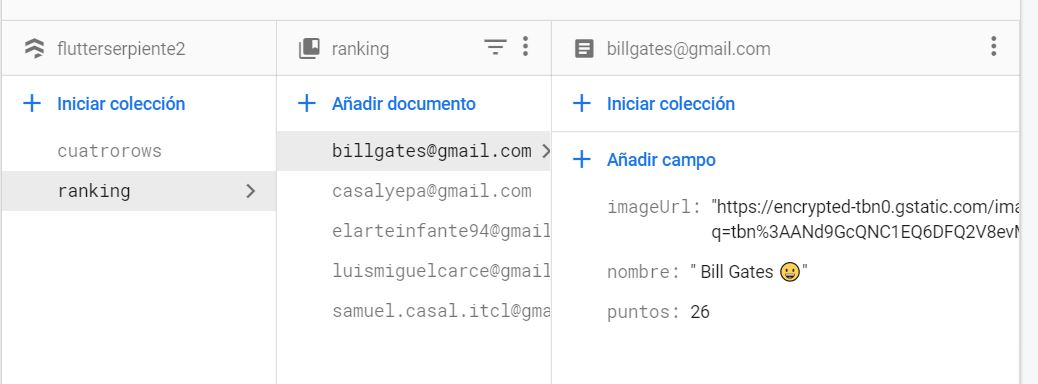
\includegraphics[width=0.9\textwidth]{disenio/firestore.jpg}
		\caption{Base de datos en firestore}\label{fig:firestore}
	\end{figure}

	\item \textbf{Sqlflite:} esta base de datos si que sigue el modelo tradicional del SGBDR. En mi caso fue necesario usar este paquete~\cite{package:sqlflite}, que internamente funciona con sqlite. Usado para almacenar datos en forma local, ya que no era necesario que los datos salieran del terminal.
	
	
\end{itemize}

\section{Diseño procedimental}

\section{Diseño arquitectónico}


